\documentclass[a4j, titlepage]{jsarticle}
\usepackage[dvipdfmx]{graphicx}
\usepackage{amsmath,ascmac,amsthm, amssymb}
\usepackage{amsfonts,latexsym,mathtools}
\usepackage{bm}
\usepackage{algorithm,algorithmic}
\usepackage{listings}
\usepackage{empheq}
\lstset{
    language={C},
    basicstyle={\small\ttfamily},
    identifierstyle={\small},
    commentstyle={\small\itshape},
    keywordstyle={\small\bfseries},
    ndkeywordstyle={\small},
    stringstyle={\small\ttfamily},
    frame={tb},
    breaklines=true,
    columns=[l]{fullflexible},
    numbers=left,
    xrightmargin=0zw,
    xleftmargin=3zw,
    numberstyle={\scriptsize},
    stepnumber=1,
    numbersep=1zw,
    lineskip=-0.5ex
}
\renewcommand{\lstlistingname}{コード}
\renewcommand{\lstlistlistingname}{コード目次}

\numberwithin{equation}{section}
%\setcounter{tocdepth}{3}

\begin{document}
\begin{titlepage}
    \begin{center}
        {\Large 令和四年度後期 数理工学実験 課題レポート}

        \vspace*{180truept}

        {\Huge 常微分方程式の数値解法}

        \vspace{160truept}

        {\Large 情報学科2回生 平田蓮}

        \vspace{10truept}

        {\large 学生番号: 1029342830}

        \vspace{60truept}

        {\large 実験日: 10月11, 17, 18, 24日}

        \vspace{10truept}

        {\large 実験場所: 京都大学工学部総合校舎数理計算機室}

        \vspace{60truept}

        {\large 10月31日 提出}
    \end{center}
\end{titlepage}

\tableofcontents
\clearpage

\section{目的}
    多くの数理モデルには、微分方程式が現れる。
    これの解を解析的に得ることは一般的には難しいため、
    数値計算でその近似解求めるためのアルゴリズムを学習する。

\section{原理}
    本章では、続く課題で用いるアルゴリズムについて述べる。

    \subsection{オイラー法}
        以下の関数を考える。
        \begin{equation}
            \frac{\mathrm{d}u}{\mathrm{d}t}(t) = f(t, u(t)), \ u(0) = u_0 \label{equ:diff}
        \end{equation}
        この式の両辺を$t$について、$[t_a, t_b]$の範囲で積分すると、
        \begin{equation*}
            u(t_b) - u(t_a) = \int^{t_b}_{t_a}f(t, u(t))\mathrm{d}t
        \end{equation*}
        を得る。$\Delta t = t_b - t_a$とすると、
        範囲内の積分を幅$\Delta t$、高さ$f(t_a, u(t_a))$の
        長方形の面積で近似でき、
        \begin{alignat*}{2}
            & u(t_b) - u(t_a) & \ \approx \ & f(t_a, u(t_a))\Delta t \\
            \rightarrow \ & u(t_b) & \ \approx \ & u(t_a) + f(t_a, u(t_a))\Delta t
        \end{alignat*}
        と書ける。ここで$(a, b)$を$(n, n + 1)$に置き換え、
        さらに$u(t_n)$を$u_n$に書き換えると、
        \begin{equation}
            u_{n + 1} \approx u_n + f(t_n, u_n)\Delta t \label{equ:euler}
        \end{equation}
        を得る。この式を$n$に対して繰り返し適用することで、
        式(\ref{equ:diff})を満たす関数を数値計算することができる。

        式(\ref{equ:euler})は積分の近似の際に$f(t_a, u(t_a))$を用いたが、
        $f(t_b, u(t_b))$を用いても同様に近似でき、
        前者を前進オイラー法、後者を後退オイラー法と呼ぶ。

    \subsection{クランク・ニコルソン法} \label{sec:crank}
        オイラー法では$[t_n, t_{n+1}]$の積分を長方形の面積で近似したが、
        範囲内の関数を1次関数で近似することで、台形の面積で近似でき、
        精度を向上させることができる。台形で近似を行うと、
        \begin{equation}
            u_{n + 1} \approx u_n + \frac{f(t_n, u_n) + f(t_{n+1}, u_{n+1})}{2}\Delta t \label{equ:crank}
        \end{equation}
        を得る。この式は、$u_{n+1}$の近似が$u_{n+1}$を用いて陰的に表されている陰解法であるため、
        そのまま計算するには工夫が必要である。

    \subsection{アダムス・バッシュフォース法}
        オイラー法やクランク・ニコルソン法では、$u_{n+1}$を求める際に$u_{n}$のみを用いるため、
        一段法と呼ばれる。対して、$u_{n-1}$や$u_{n-2}$など、
        より過去の値も用いて精度を高めるアルゴリズムを多段法と呼ぶ。

        過去に計算した$N+1$個の点
        を用いてラグランジュ補間により式(\ref{equ:diff})を満たす$f(t, u(t))$を
        $N$次多項式で構成することを考える。

        \subsubsection{$N=1$の場合}
            まず、1次式で近似する場合を考える。
            すでに計算した2点
            $(t_n, f(t_n, u_n))$,
            $(t_{n-1}, f(t_{n-1}, u_{n-1}))$
            を用いてラグランジュ補完を行うと、
            \begin{equation*}
                f(t, u(t)) \approx \frac{t - t_{n-1}}{t_n - t_{n-1}}f(t_n, u_n) + \frac{t - t_n}{t_{n-1} - t_n}f(t_{n-1}, u_{n-1})
            \end{equation*}
            を得る。$t_n - t_{n-1} = \Delta t$を踏まえると、
            \begin{eqnarray*}
                f(t, u(t)) &\approx& \frac{t - t_{n-1}}{\Delta t}f(t_n, u_n) - \frac{t - t_n}{\Delta t}f(t_{n-1}, u_{n-1}) \\
                &=& \frac{f(t_n, u_n) - f(t_{n-1}, u_{n-1})}{\Delta t}t - \frac{t_{n-1}f(t_n, u_n) - t_nf(t_{n-1}, u_{n-1})}{\Delta t}
            \end{eqnarray*}
            と書ける。これを$t_{n+1} - t_{n} = \Delta t$を踏まえて$[t_n, t_{n+1}]$の範囲で積分すると、
            \begin{eqnarray*}
                \int^{t_{n+1}}_{t_n} f(t, u(t)) dt &\approx& \int^{t_{n+1}}_{t_n} \left\{ \frac{f(t_n, u_n) - f(t_{n-1}, u_{n-1})}{\Delta t}t - \frac{t_{n-1}f(t_n, u_n) - t_nf(t_{n-1}, u_{n-1})}{\Delta t} \right\} dt \\
                &=& 2\Delta t f(t_n, u_n) - \frac{\Delta t}{2} f(t_n, u_n) - \frac{\Delta t}{2} f(t_{n-1}, u_{n-1}) \\
                &=& \frac{\Delta t}{2} \{3f(t_n, u_n) - f(t_{n-1}, u_{n-1})\}
            \end{eqnarray*}
            よって、
            \begin{equation}
                u_{n+1} \approx u_n + \frac{\Delta t}{2} \{3f(t_n, u_n) - f(t_{n-1}, u_{n-1})\}
            \end{equation}
            となる。これを2次アダムス・バッシュフォース法と呼ぶ。

        \subsubsection{$N=2$の場合}
            2次式で近似を行う場合、3点が必要である。
            $(t_n, f(t_n, u_n))$,
            $(t_{n-1}, f(t_{n-1}, u_{n-1}))$,
            $(t_{n-2}, f(t_{n-2}, u_{n-2}))$
            を用いて同様に補間を行うと、
            \begin{eqnarray*}
                f(t, u(t)) &\approx& \frac{(t - t_{n-1})(t - t_{n-2})}{(t_n - t_{n-1})(t_n - t_{n-2})}f(t_n, u_n) + \\
                && \frac{(t - t_{n-2})(t - t_n)}{(t_{n-1} - t_{n-2})(t_{n-1} - t_n)}f(t_{n-1}, u_{n-1}) + \\
                && \frac{(t - t_n)(t - t_{n-1})}{(t_{n-2} - t_n)(t_{n-2} - t_{n-1})}f(t_{n-2}, u_{n-2})
            \end{eqnarray*}
            を得る。$N=1$の場合と同様に積分を行うと、
            \begin{eqnarray}
                \int^{t_{n+1}}_{t_n} f(t, u(t)) dt &\approx& \frac{\Delta t}{12} \{23f(t_n, u_n) - 16f(t_{n-1}, u_{n-1}) + 5f(t_{n-2}, u_{n-2})\} \nonumber \\
                \therefore u_{n+1} &\approx& u_n + \frac{\Delta t}{12} \{23f(t_n, u_n) - 16f(t_{n-1}, u_{n-1}) + 5f(t_{n-2}, u_{n-2})\}
            \end{eqnarray}
            となる\cite{text}。これを3次アダムス・バッシュフォース法と呼ぶ。

    \subsection{ホイン法}
        \ref{sec:crank}節で、
        クランク・ニコルソン法を計算するには工夫が必要であると述べた。
        工夫の一つとして、$f(t_{n+1},u_{n+1})$を$u_n$と$f(t_n, u_n)$を用いて表すことを考える。
        オイラー法を用いると、
        \begin{equation*}
            u_{n+1} = u_n + f(t_n, u_n)\Delta t
        \end{equation*}
        と書ける。これを式(\ref{equ:crank})に代入すると、
        \begin{eqnarray}
            u_{n+1} &\approx& u_n + \frac{f(t_n, u_n) + f(t_{n+1}, u_n + f(t_n, u_n)\Delta t)}{2}\Delta t \label{equ:heun}
        \end{eqnarray}
        を得る。これをホイン法と呼び、
        $u_{n+1}$の近似が$u_n$のみによって陽的に表されている陽解法である。

    \subsection{ルンゲ・クッタ法}
        ホイン法は2次の一段法であるが、これを4次に拡張したものを4次ルンゲ・クッタ法と呼び、
        これは以下の式で表される。
        \begin{eqnarray}
            u_{n+1} &=& u_n + \frac{F_1 + 2F_2 + 2F_3 + F_4}{6} \\
            &&\begin{cases}
                F_1 = f(t_n, u_n) \\
                F_2 = \displaystyle f(t_n + \frac{\Delta t}{2}, u_n + F_1\frac{\Delta t}{2}) \\
                F_3 = \displaystyle f(t_n + \frac{\Delta t}{2}, u_n + F_2\frac{\Delta t}{2}) \\
                F_4 = f(t_{n+1}, u_n + F_3\Delta t)
            \end{cases}
        \end{eqnarray}

        これの証明は膨大な記述量であるため、ここでは省略する。
        詳細は\cite{runge}を参照されたい。

\section{課題} \label{sec:ex}
    \subsection{課題3 常微分方程式の数値解}
        式(\ref{equ:3diff})で表される常微分方程式の初期値問題を考える。
        \begin{equation}
            \frac{\mathrm{d}u}{\mathrm{d}t}=u, \ u(0)=1 \label{equ:3diff}
        \end{equation}
        ステップ幅を$\Delta t$として、$t$での数値解を$u_\mathrm{calc}(t, \Delta t)$とする。
        $t=1$において、数値解$u_\mathrm{calc}(1, \Delta t)$と厳密解$u(1)$の差を
        \begin{equation}
            E(\Delta t) = |u_\mathrm{calc}(1, \Delta t) - u(1)| \label{equ:3loss}
        \end{equation}
        とする。

        以下に示すアルゴリズムについて、式(\ref{equ:3loss})の関数形を調べる。
        \begin{itemize}
            \item 前進オイラー法 (FE)
            \item 2次アダムス・バッシュフォース法 (AB2)
            \item 3次アダムス・バッシュフォース法 (AB3)
            \item ホイン法 (H)
            \item 4次ルンゲ・クッタ法 (RK)
        \end{itemize}

        \subsubsection{結果}
            描画したグラフを以下に示す。
            \paragraph{前進オイラー法}
                \begin{center}
                    \begin{figure}[h]
                        \centering
                        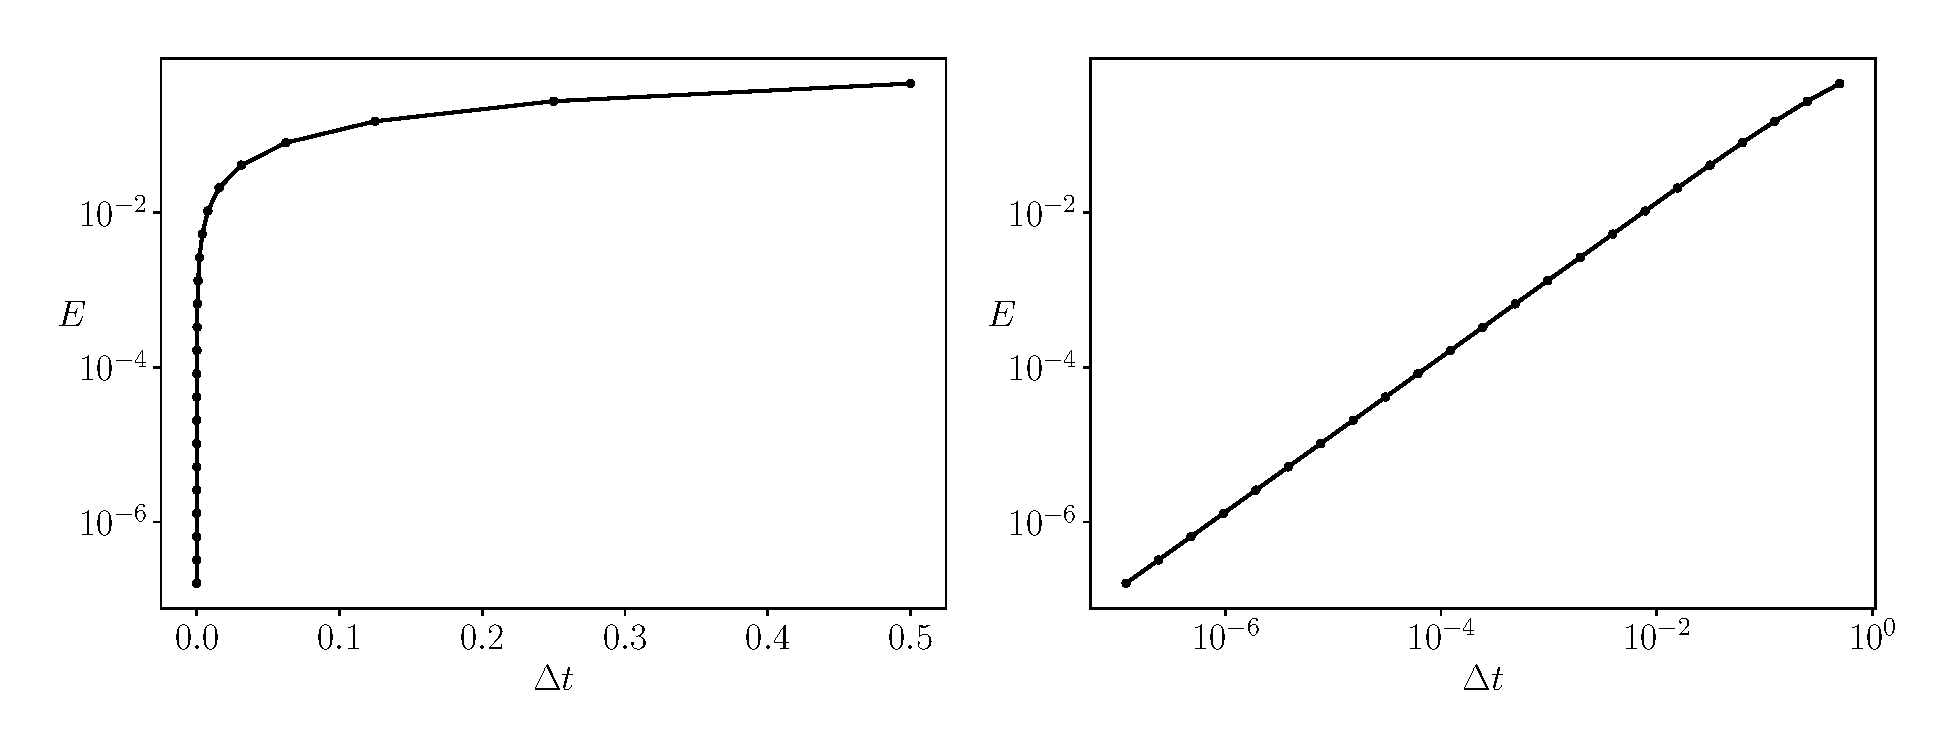
\includegraphics[width=1\hsize]{kadai3/euler.eps}
                        \caption{
                            前進オイラー法を用いて計算した$E(\Delta t)$。
                            左は片対数、右は両対数グラフ
                        }
                    \end{figure}
                \end{center}

            \paragraph{2次アダムス・バッシュフォース法}
                \begin{center}
                    \begin{figure}[h]
                        \centering
                        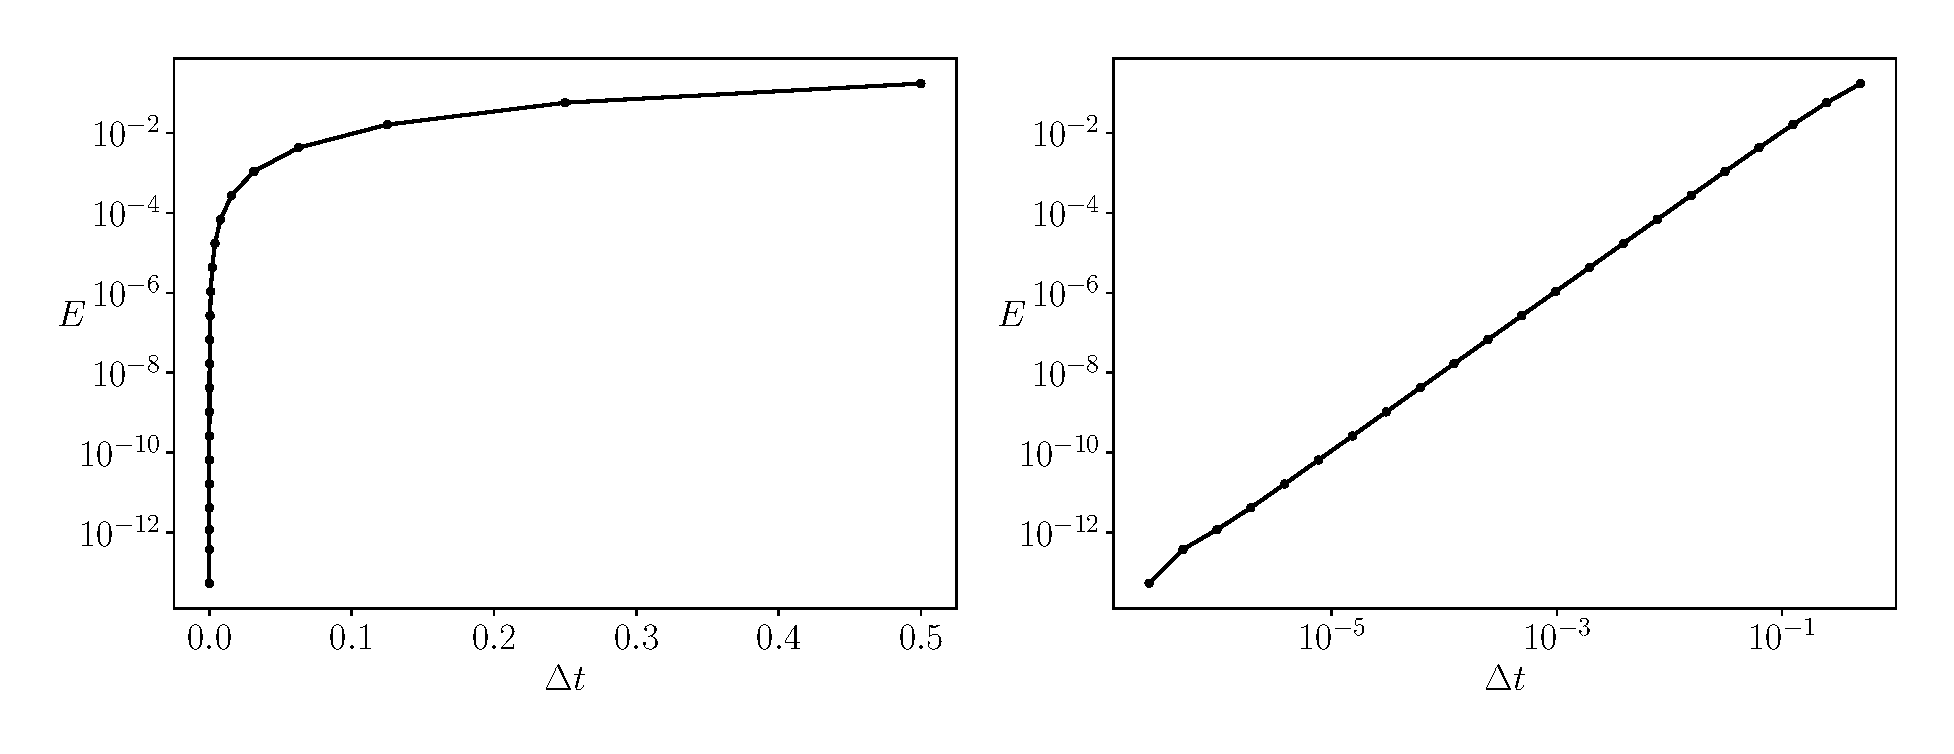
\includegraphics[width=1\hsize]{kadai3/ab2.eps}
                        \caption{
                            2次アダムス・バッシュフォース法を用いて計算した$E(\Delta t)$。
                            左は片対数、右は両対数グラフ
                        }
                    \end{figure}
                \end{center}

            \paragraph{3次アダムス・バッシュフォース法}
                \begin{center}
                    \begin{figure}[h]
                        \centering
                        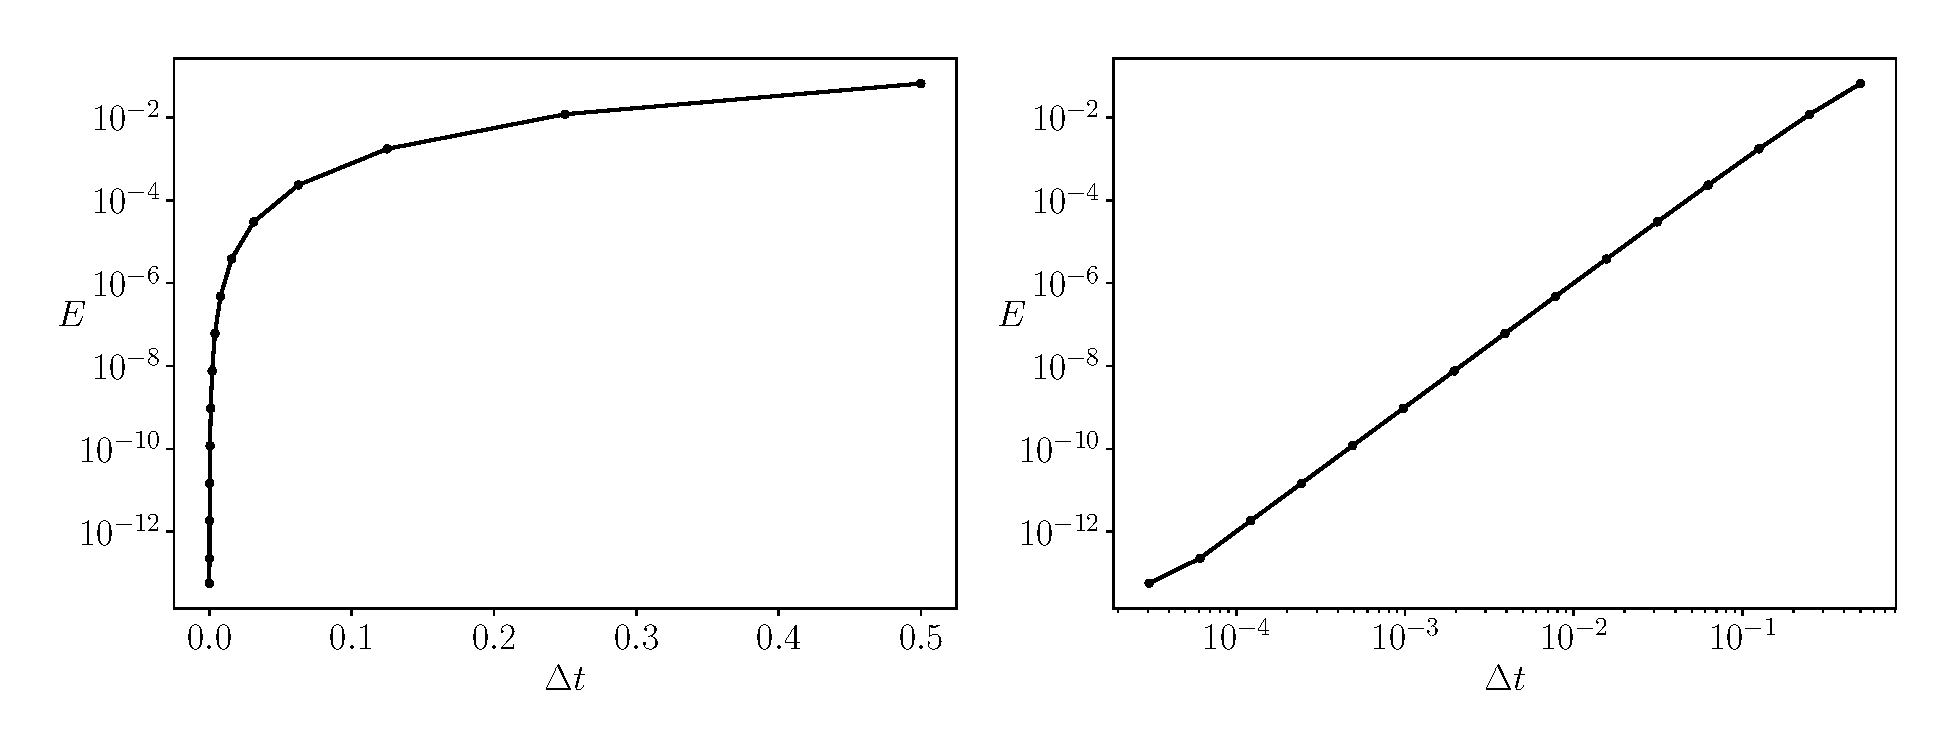
\includegraphics[width=1\hsize]{kadai3/ab3.eps}
                        \caption{
                            3次アダムス・バッシュフォース法を用いて計算した$E(\Delta t)$。
                            左は片対数、右は両対数グラフ
                        }
                    \end{figure}
                \end{center}

            \paragraph{ホイン法}
                \begin{center}
                    \begin{figure}[h]
                        \centering
                        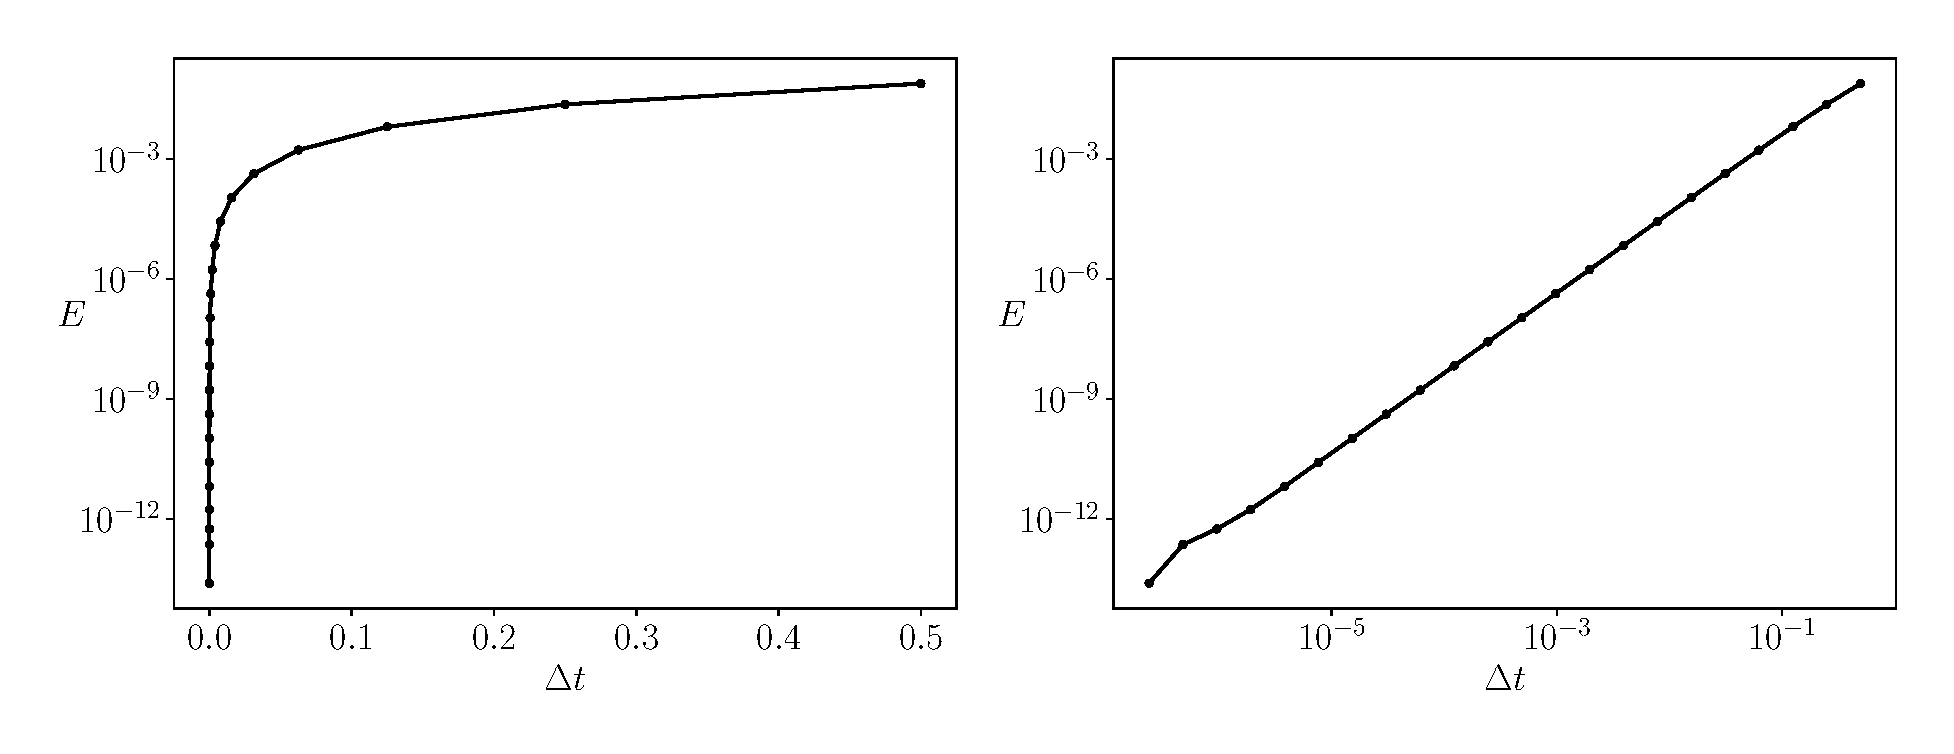
\includegraphics[width=1\hsize]{kadai3/heun.eps}
                        \caption{
                            ホイン法を用いて計算した$E(\Delta t)$。
                            左は片対数、右は両対数グラフ
                        }
                    \end{figure}
                \end{center}

            \paragraph{4次ルンゲ・クッタ法}
                \begin{center}
                    \begin{figure}[h]
                        \centering
                        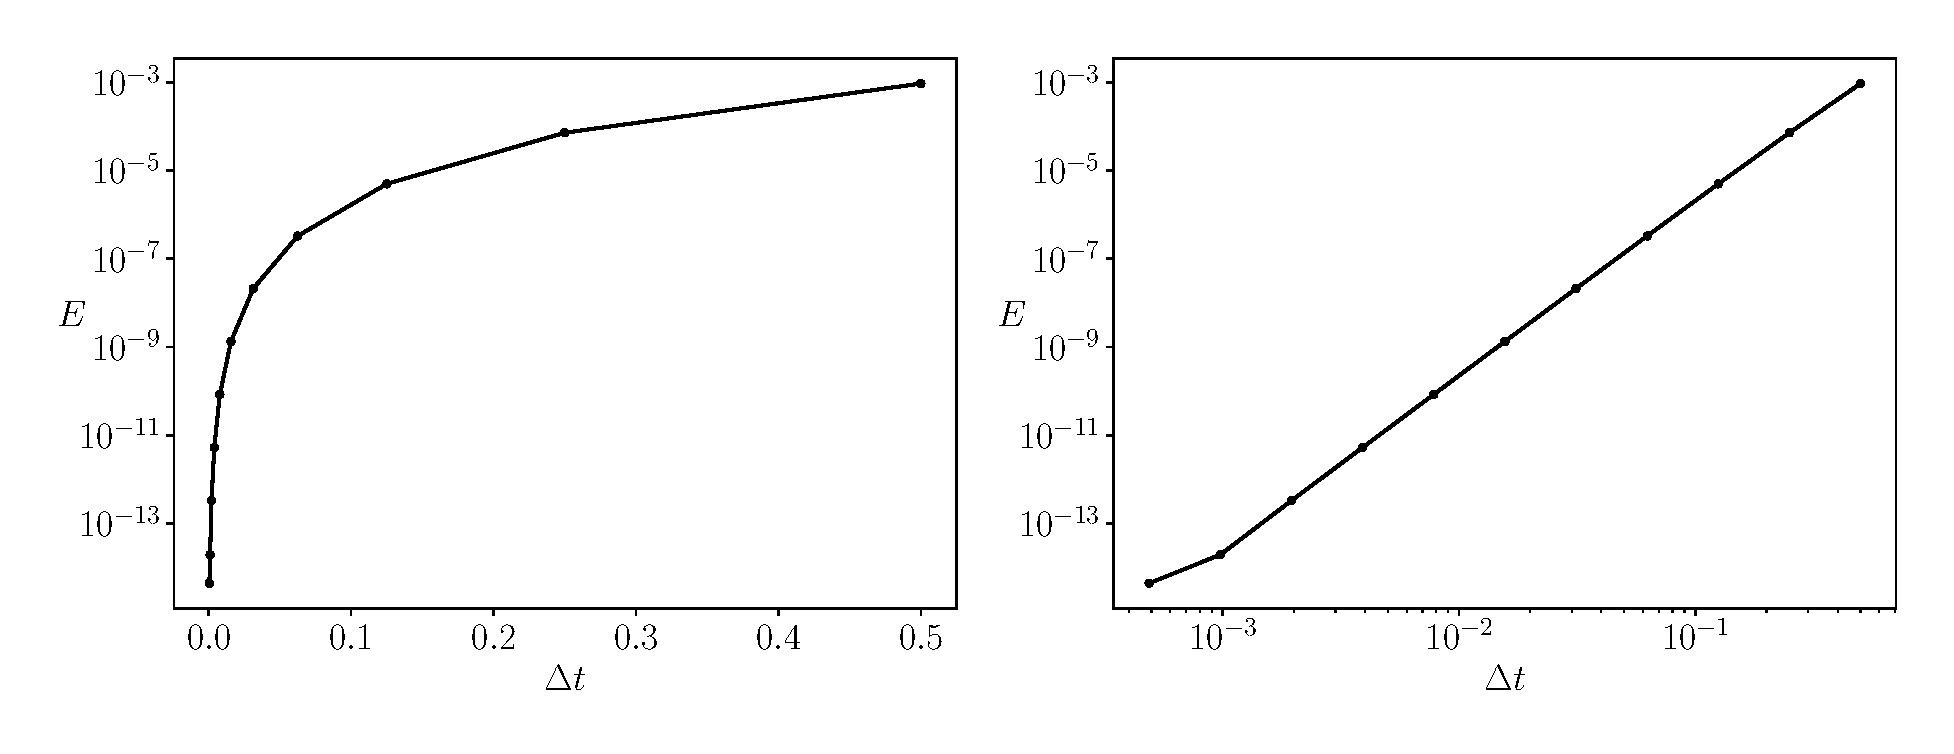
\includegraphics[width=1\hsize]{kadai3/runge_kutta.eps}
                        \caption{
                            4次ルンゲ・クッタ法を用いて計算した$E(\Delta t)$。
                            左は片対数、右は両対数グラフ
                        }
                    \end{figure}
                \end{center}

        \subsubsection{考察}
            どのアルゴリズムを用いて計算した$E(\Delta t)$も、
            両対数グラフでは直線に近似していることがわかる。
            このことから、$E(\Delta t)$の関数形は全て冪関数であることがわかる。
            次に、この冪関数それぞれの指数について考える。
            $n$次のアルゴリズムでは、1ステップあたりの数値解と厳密解の差は
            $O(\Delta t^{n + 1})$であるので、
            $N=\displaystyle\frac{1}{\Delta t}$ステップ計算した際の差は、
            \begin{equation}
                O(N\times\Delta t^{n + 1}) = O\left(\frac{1}{\Delta t}\times\Delta t^{n + 1}\right) = O(\Delta t^n) \label{equ:guess}
            \end{equation}
            になると予想できる。

            図\ref{fig:3}に、両対数グラフに上のグラフをまとめたものを示す。
            \begin{figure}[h]
                \centering
                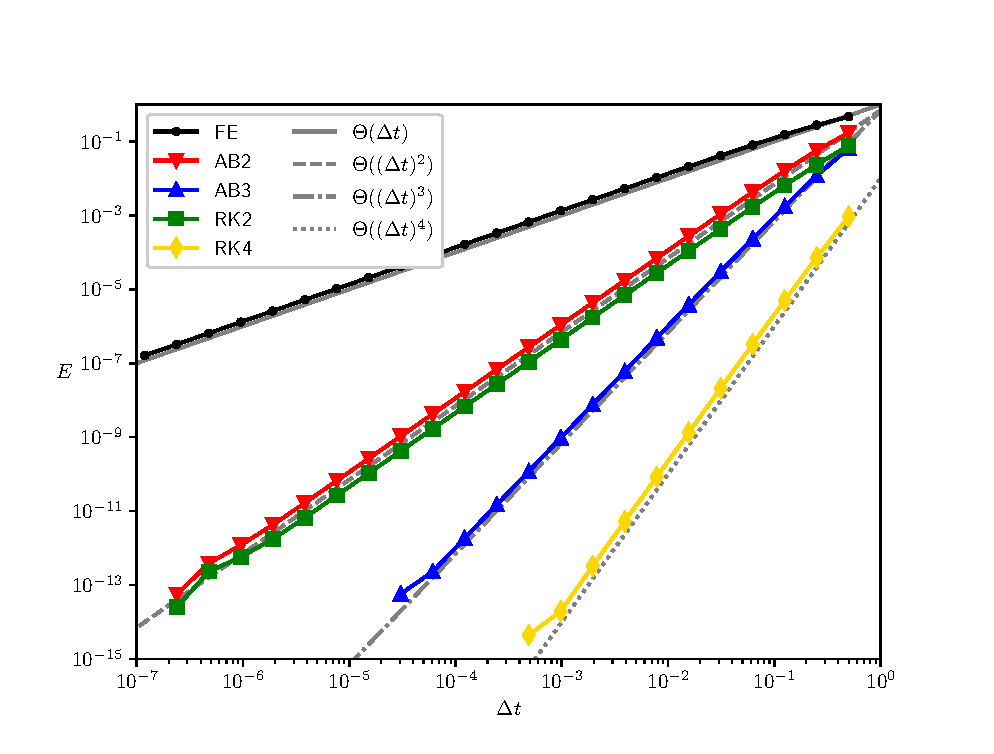
\includegraphics[width=0.8\hsize]{kadai3/kadai3.eps}
                \caption{
                    それぞれのアルゴリズムで計算した$E(\Delta t)$ (両対数グラフ)。
                    $E(\Delta t)$の他に、$n=1,2,3,4$について、
                    $\Theta(\Delta t^n)$のグラフを重ねた。
                }
                \label{fig:3}
            \end{figure}
            それぞれのアルゴリズムで計算した$E(\Delta t)$と、
            $\Theta(\Delta t^n)$の傾きを比較することで$E(\Delta t)$の指数を観測することができる。
            例えば、ホイン法の$E(\Delta t)$と$\Theta(\Delta t^2)$は傾きが等しいため、
            定数$A$を用いて$E(\Delta t) = A\Delta t^2$と書けることがわかる。
            これを、式(\ref{equ:guess})に示した予測とともにまとめると表\ref{tab:3}
            のようになり、予測が正しかったことがわかる。

            \begin{table}[h]
                \centering
                \caption{
                    $E(\Delta t)$の指数の予測と計算結果
                }
                \label{tab:3}
                \begin{tabular}{c|rrr} \hline
                    アルゴリズム & アルゴリズムの次数 & 予測される指数 & 実際の指数 \\ \hline \hline
                    オイラー法 & 1 & 1 & 1 \\
                    2次アダムス・バッシュフォース法 & 2 & 2 & 2 \\
                    3次アダムス・バッシュフォース法 & 3 & 3 & 3 \\
                    ホイン法 & 2 & 2 & 2 \\
                    4次ルンゲ・クッタ法 & 4 & 4 & 4 \\ \hline
                \end{tabular}
            \end{table}

        \subsubsection{結論}
            本課題で用いた5つのアルゴリズムでは、
            $E(\Delta t)$の関数形は全て冪関数となり、
            その指数はアルゴリズムの次数と等しくなることがわかった。

    \subsection{課題4 陰・陽解法の安定性}
        微分方程式の数値解法の安定性について考える。
        ここで、アルゴリズムが安定であることと、
        $\displaystyle\lim_{t\to\infty}|u(t)|\neq\infty$
        となることは同じとする。アルゴリズムの差分式が
        式(\ref{equ:rec})の漸化式で表される場合を考える。
        \begin{equation}
            u_{n+1} = au_n+b \ (a\neq 1) \label{equ:rec}
        \end{equation}
        
        これの一般項は、$u$の初期値$u_0$を用いて、
        \begin{equation}
            u_n = \left(u_0-\frac{b}{1-a}\right)a^n+\frac{b}{1-a}
        \end{equation}
        で与えられる\cite{2rec}。アルゴリズムが安定であるとき、
        $\displaystyle\lim_{n\to\infty}u_n\neq\infty$であるので、
        $|a|<1$であればアルゴリズムは安定であるといえる。

        これを踏まえて、式(\ref{equ:4diff})に示す常微分方程式における
        以下に示すアルゴリズムの安定性を調べる。
        \begin{equation}
            \frac{\mathrm{d}u}{\mathrm{d}t} = -\alpha u + \beta, \ u(0) = u_0, \ \alpha > 0, \beta \in \mathbb{R} \label{equ:4diff}
        \end{equation}
        \begin{itemize}
            \item クランク・ニコルソン法 (陰解法)
            \item ホイン法 (陽解法)
        \end{itemize}

        \subsubsection{クランク・ニコルソン法の安定性} \label{sec:4crank}
            式(\ref{equ:crank})に式(\ref{equ:4diff})を代入すると、
            \begin{eqnarray*}
                u_{n + 1} &\approx& u_n + \frac{(-\alpha u_n + \beta) + (-\alpha u_{n + 1} + \beta)}{2}\Delta t \\
                \rightarrow u_{n + 1} &\approx& \frac{2 - \alpha\Delta t}{2 + \alpha\Delta t}u_n + \frac{2\beta}{2 + \alpha\Delta t}\Delta t
            \end{eqnarray*}
            を得る。上に示したように、
            $\displaystyle\left|\frac{2 - \alpha\Delta t}{2 + \alpha\Delta t}\right| < 1$
            となればアルゴリズムは安定といえる。
            仮定より$\alpha, \Delta t > 0$であるため、
            これは常に満たされ、このアルゴリズムは常に安定であるといえる。

        \subsubsection{ホイン法の安定性}
            式(\ref{equ:heun})に式(\ref{equ:4diff})を代入すると、
            \begin{eqnarray*}
                u_{n + 1} &\approx& u_n + \frac{(-\alpha u_n + \beta) + [-\alpha \{u_n + (-\alpha u_n + \beta)\Delta t\} + \beta]}{2}\Delta t \\
                \rightarrow u_{n + 1} &\approx& \left(1 - \alpha\Delta t + \frac{\alpha^2\Delta t^2}{2}\right)u_n + \left(1 - \frac{\alpha\Delta t}{2}\right)\beta\Delta t
            \end{eqnarray*}
            を得る。\ref{sec:4crank}節と同様に、
            $\displaystyle\left|1 - \alpha\Delta t + \frac{\alpha^2\Delta t^2}{2}\right| < 1$
            となればアルゴリズムは安定といえる。式変形を行うと、
            \begin{eqnarray}
                &&\left|1 - \alpha\Delta t + \frac{\alpha^2\Delta t^2}{2}\right| < 1 \nonumber \\
                &\rightarrow& 0 < (2 - \alpha\Delta t)\alpha\Delta t < 4 \label{equ:4heun}
            \end{eqnarray}
            となるため、$0 < (2 - \alpha\Delta t)\alpha\Delta t < 4$を満たす$\Delta t$について、
            アルゴリズムは安定であるといえる。

        \subsubsection{数値計算による確認} \label{sec:4calc}
            $u_0 = 1, \alpha = 10, \beta = 1$として、
            上で述べた結果を数値計算により確認する。
            計算した結果を図\ref{fig:4crank}, \ref{fig:4heun}に示す。
            \begin{figure}[h]
                \begin{minipage}{0.49\hsize}
                    \centering
                    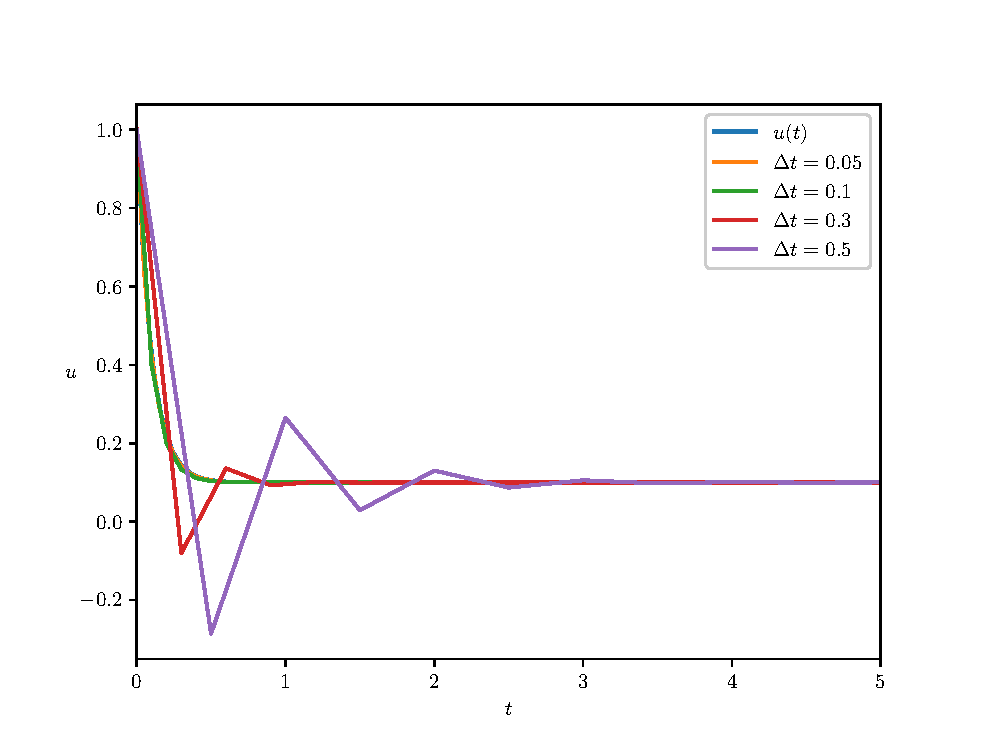
\includegraphics[width=1\hsize]{kadai4/crank.eps}
                    \caption{
                        クランク・ニコルソン法による
                        式(\ref{equ:4diff})の数値計算結果。
                        $\Delta t = 0.1, 0.3, 0.5$の場合の結果と、
                        理論値をプロットした。
                    }
                    \label{fig:4crank}
                \end{minipage}
                \begin{minipage}{0.49\hsize}
                    \centering
                    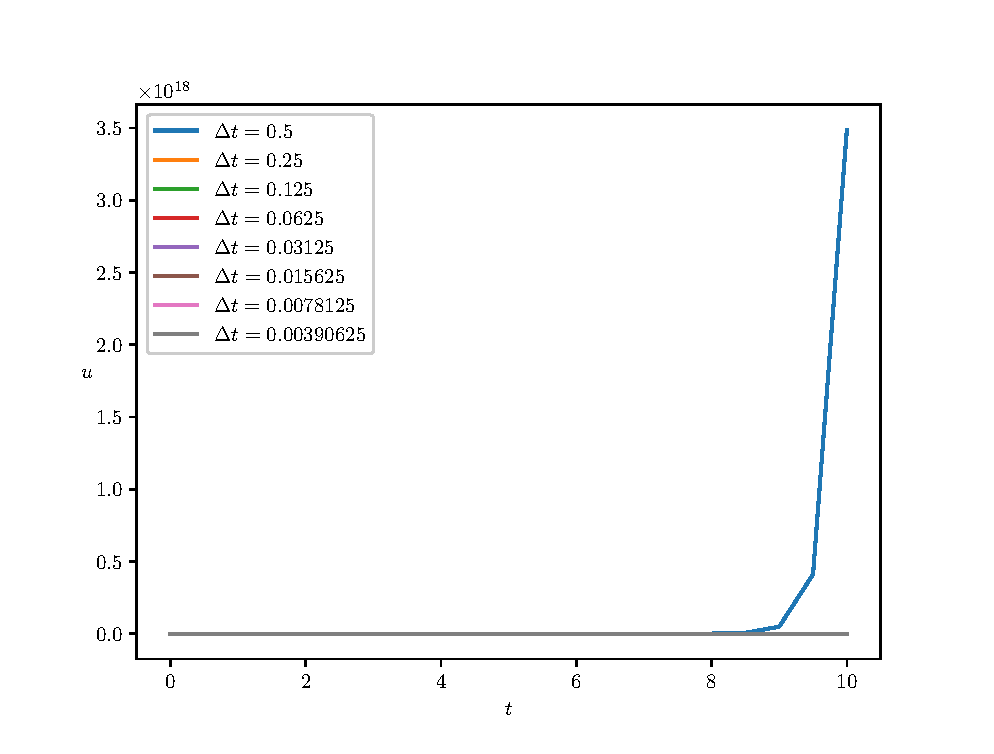
\includegraphics[width=1\hsize]{kadai4/heun.eps}
                    \caption{
                        ホイン法による数値計算結果。式(\ref{equ:4diff})の数値計算結果。
                        $\Delta t = 0.05, 0.15, 0.21$の場合の結果と、
                        理論値をプロットした。
                    }
                    \label{fig:4heun}
                \end{minipage}
            \end{figure}

        \subsubsection{考察}
            \ref{sec:4crank}節での予測通り、クランク・ニコルソン法は、
            $\Delta t$を増大させても安定なアルゴリズムであることが図\ref{fig:4crank}
            より見てとれる。
            一方、図\ref{fig:4heun}を見ると、
            ホイン法は$\Delta t=0.21$の際に計算結果が発散し、
            不安定になっている。

            式(\ref{equ:4heun})に\ref{sec:4calc}節で示したパラメータを代入すると、
            \begin{eqnarray*}
                && 0 < (2 - 10\Delta t)\times 10\Delta t < 4 \\
                &\rightarrow& 0 < (0.2 - \Delta t)\times \Delta t < 0.04 \\
                &\rightarrow& 0 < \Delta t < 0.2
            \end{eqnarray*}
            を得る。実際に、$\Delta t = 0.21 > 0.2$で発散が起こっているため、
            \ref{sec:4calc}節での予測は正しかったことになる。

        \subsubsection{結論}
            陰解法であるクランク・ニコルソン法では$\Delta t$を変化させても
            アルゴリズムが不安定になることはなかったが、
            陽解法であるホイン法を用いると、
            $\Delta t$が一定の大きさを超えた際に不安定になることがわかった。

    \subsection{課題5 アルゴリズムの安定性}
        式(\ref{equ:5diff})で表される方程式を考える。
        \begin{equation}
            \frac{\mathrm{d}u}{\mathrm{d}t} = -2u + 1 \label{equ:5diff}
        \end{equation}
        これの厳密解を求める。式変形を行うと、
        \begin{eqnarray*}
            \frac{\mathrm{d}u}{\mathrm{d}t} &=& -2u + 1 \\
            \rightarrow \frac{\mathrm{d}u}{-2u + 1} &=& \mathrm{d}t
        \end{eqnarray*}
        となる。両辺を積分すると、
        \begin{eqnarray*}
            \int\frac{\mathrm{d}u}{-2u + 1} &=& \int\mathrm{d}t \\
            \rightarrow -\frac{1}{2}\ln|-2u + 1| &=& t + C \ (Cは定数) \\
            \rightarrow -2u + 1 &=& \pm e^{-2t - 2C} \\
            &=& C'e^{-2t} \ (C' \coloneqq \pm e^{-2C}) \\
            \rightarrow u &=& -\frac{C'e^{-2t} - 1}{2} \\
            &=& C''e^{-2t} + \frac{1}{2} \ \left(C'' \coloneqq -\frac{C'}{2}\right)
        \end{eqnarray*}
        を得る。これの初期値$u(0)$は$C''$によって決まるが、
        $t \rightarrow \infty$において$\left|e^{-2t}\right|\rightarrow\infty$であるので、
        $u$は任意の初期値について$t\rightarrow\infty$で$\displaystyle\frac{1}{2}$に収束する。

        \subsubsection{アルゴリズムの安定性} \label{sec:alg_stable}
            式(\ref{equ:5alg})に示すアルゴリズムを用いて式(\ref{equ:5diff})に示した方程式の
            解を数値計算することを考える。
            \begin{equation}
                u_n = u_{n - 2} + 2f(t_{n - 1}, u_{n - 1})\Delta t \label{equ:5alg}
            \end{equation}
            これに式(\ref{equ:5diff})を代入すると、
            \begin{eqnarray*}
                && u_n = u_{n - 2} + 2(-2u_{n - 1} + 1)\Delta t \\
                &\rightarrow& u_n = u_{n - 2} - 4u_{n - 1}\Delta t + 2\Delta t
            \end{eqnarray*}
            を得る。これの一般項は、定数$C_1, C_2$を用いて、
            \begin{equation*}
                u_n = C_1\left(-\sqrt{4\Delta t^2 + 1}-2\Delta t\right)^n + C_2\left(\sqrt{4\Delta t^2 + 1}-2\Delta t\right)^n + \frac{1}{2}
            \end{equation*}
            と表せる\cite{3rec}。
            $n\rightarrow\infty$について、これが安定なアルゴリズムであるためには、
            \begin{empheq}[left={\empheqlbrace}]{align}
                &\left|-\sqrt{4\Delta t^2 + 1}-2\Delta t\right| < 1 \label{equ:5alg_stable1} \\
                &\left|\sqrt{4\Delta t^2 + 1}-2\Delta t\right| < 1 \nonumber
              \end{empheq}
            を同時に満たす必要がある。

            式(\ref{equ:5alg_stable1})を変形すると、
            \begin{eqnarray*}
                && \left|-\sqrt{4\Delta t^2 + 1}-2\Delta t\right| < 1 \\
                &\rightarrow& -1 < -\sqrt{4\Delta t^2 + 1} - 2\Delta t < 1 \\
                &\rightarrow& -1 + 2\Delta t < -\sqrt{4\Delta t^2 + 1} < 1 + 2\Delta t \\
            \end{eqnarray*}
            となる。右の不等号については、$\Delta t > 0$より、常に成り立つ。
            左の不等式は、同様の理由により$\Delta t \geq 0.5$の場合に成り立たないことがわかる。
            $\Delta t < 0.5$の場合を考えると、
            \begin{eqnarray*}
                -1 + 2\Delta t &<& -\sqrt{4\Delta t^2 + 1} \\
                \rightarrow (-1 + 2\Delta t)^2 = 1 - 4\Delta t + 4\Delta t^2 &>& 4\Delta t^2 + 1 \\
                \rightarrow - 4\Delta t &>& 0
            \end{eqnarray*}
            となり、これを満たす$\Delta t$は存在しないことがわかる。
            よって、式(\ref{equ:5alg})に示したアルゴリズムでは
            式(\ref{equ:5diff})の方程式の安定解を得ることは不可能である。

        \subsubsection{数値計算による確認}
            実際に、式(\ref{equ:5alg})に示したアルゴリズムを用いて式(\ref{equ:5diff})の方程式
            の解を$\Delta t$を変化させながら数値計算した様子を図\ref{fig:5}に示す。
            初期値は$u_0 = 1$とした。
            \begin{figure}[h]
                \centering
                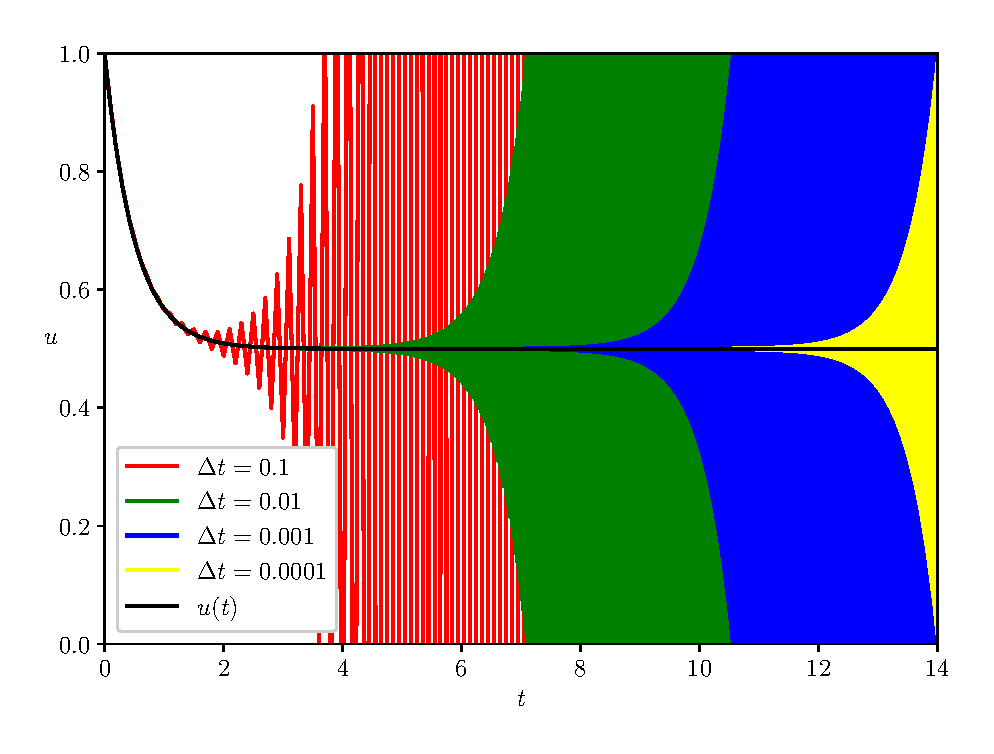
\includegraphics[width=0.8\hsize]{kadai5/kadai5.eps}
                \caption{
                    式(\ref{equ:5diff})の方程式の数値解。
                    $\Delta t = 0.1, 0.01, 0.001, 0.0001$の場合と、
                    厳密解をプロットした。
                }
                \label{fig:5}
            \end{figure}

            図より、$\Delta t$を小さくすれど、
            $t$が増加するにつれて数値解が発散していることがわかり、
            \ref{sec:alg_stable}節で述べた予測が正しかったといえる。

        \subsubsection{結論}
            式(\ref{equ:5alg})に示したアルゴリズムを用いた場合、
            式(\ref{equ:5diff})の方程式の安定解を得ることは不可能であることがわかった。

    \subsection{課題7 ローレンツ方程式}
        式(\ref{equ:laurents})で表されるローレンツ方程式を考える。
        \begin{equation}
            \begin{cases}
                \displaystyle\frac{\mathrm{d}x}{\mathrm{d}t} = \sigma(y-x) \\
                \displaystyle\frac{\mathrm{d}y}{\mathrm{d}t} = rx - y - xz \\
                \displaystyle\frac{\mathrm{d}z}{\mathrm{d}t} = xy - bz
            \end{cases} \label{equ:laurents}
        \end{equation}
        初期値を$(x(0), y(0), z(0)) = (1 + \epsilon, 0, 0)$,
        定数を$\sigma = 10, b = \displaystyle\frac{8}{3}, r = 28$とする。
        以下では、ステップ幅$\Delta t = 0.01$の4次ルンゲ・クッタ法を用いて、
        $t\in[0, 100]$の区間について数値計算を行う。

        \subsubsection{ローレンツ方程式の描画}
            $\epsilon = 0$とし、$x(t)$および、
            $(x(t), y(t), z(t))$の$xyz$空間への描画を行う。
            結果を図\ref{fig:x}, \ref{fig:xyz}に示す。
            \begin{figure}[h]
                \begin{minipage}{0.49\hsize}
                    \centering
                    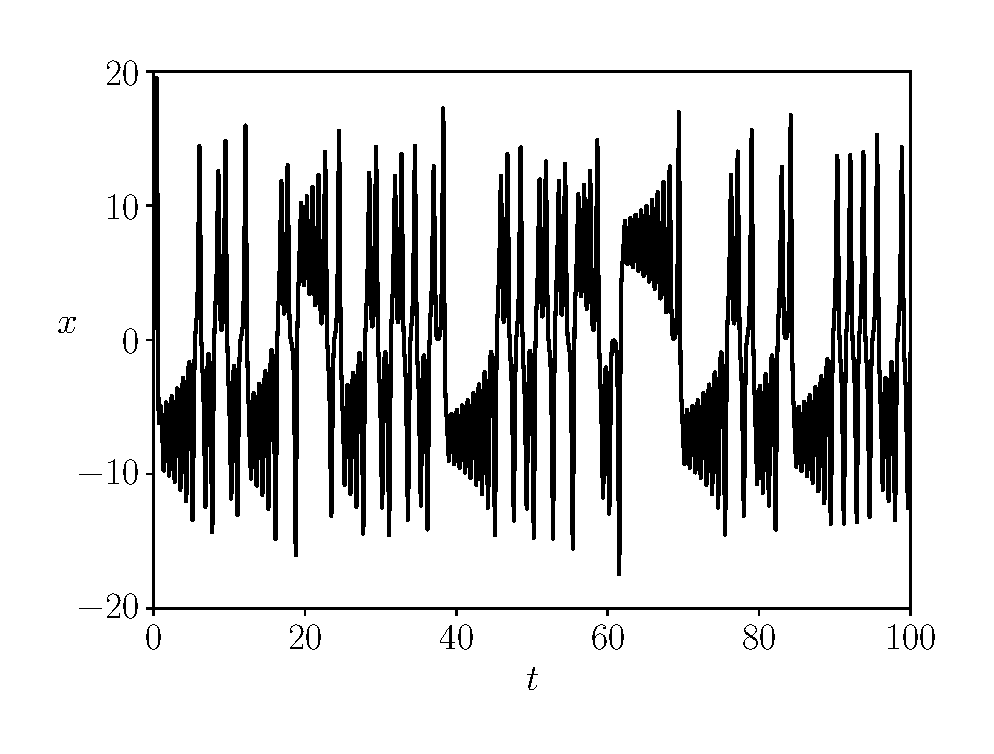
\includegraphics[width=1\hsize]{kadai7/x.eps}
                    \caption{
                        $x(t)$の数値計算結果
                    }
                    \label{fig:x}
                \end{minipage}
                \begin{minipage}{0.49\hsize}
                    \centering
                    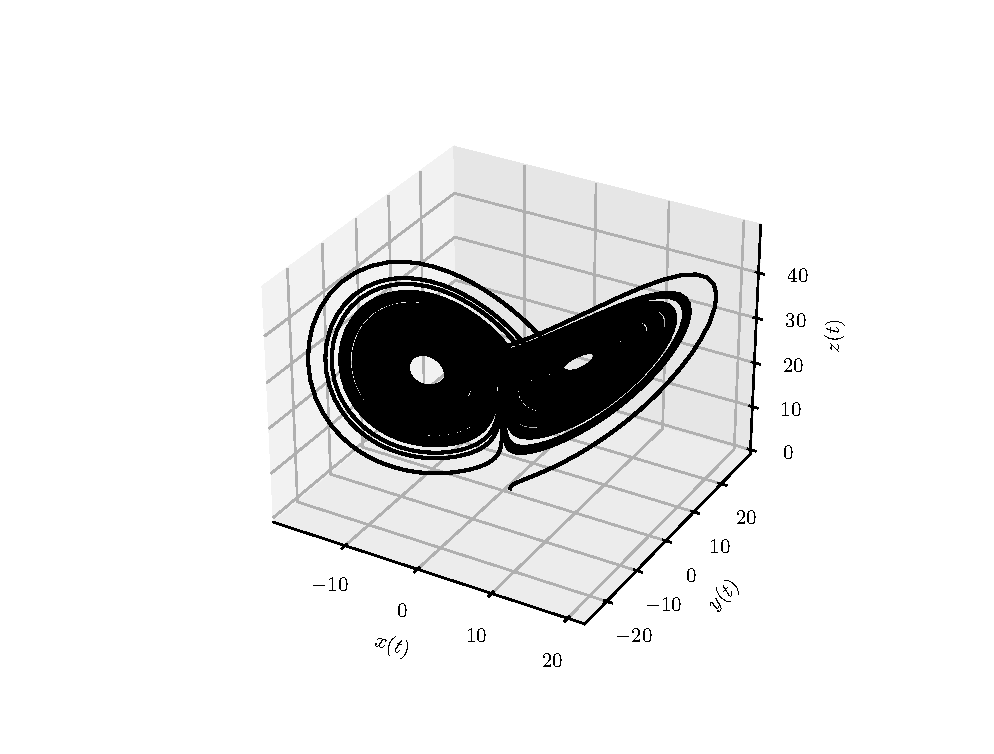
\includegraphics[width=1\hsize]{kadai7/xyz.eps}
                    \caption{
                        $(x(t), y(t), z(t))$の数値計算結果
                    }
                    \label{fig:xyz}
                \end{minipage}
            \end{figure}

        \subsubsection{$\epsilon$の変化による軌道の変化}
            $\epsilon = 0$の場合と
            $\epsilon = 10^{-n} \ (n = 2, 4, 6)$の場合の解をそれぞれ
            \begin{eqnarray*}
                \bm{x}_0(t) &=& (x_0(t), y_0(t), z_0(t)) \\
                \bm{x}_n(t) &=& (x_n(t), y_n(t), z_n(t))
            \end{eqnarray*}
            とし、これらの差
            \begin{equation*}
                \Delta_n(t) \coloneqq \|\bm{x}_0(t) - \bm{x}_n(t)\|
            \end{equation*}
            を定義する。$\Delta_n(t)$のグラフを作成し、
            これが漸近値に至る少し前の時間帯の関数形を調べる。

        \subsubsection{結果}
            $\Delta_n(t)$の計算結果を図\ref{fig:7halflog}, \ref{fig:7fulllog}に示す。
            \begin{figure}[h]
                \begin{minipage}{0.49\hsize}
                    \centering
                    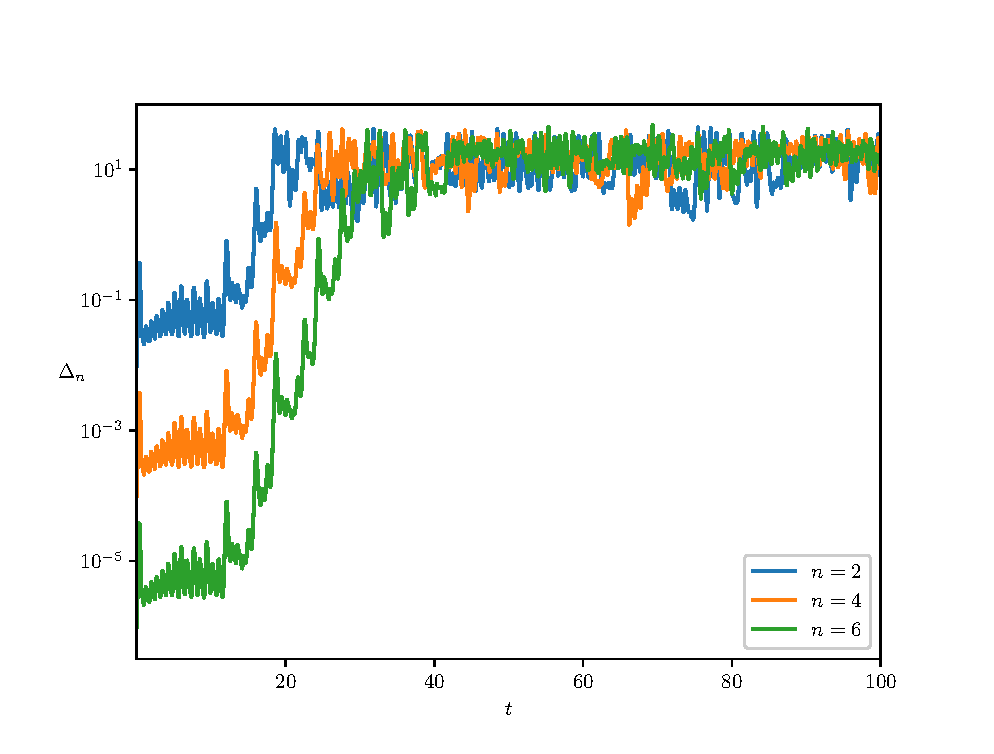
\includegraphics[width=1\hsize]{kadai7/2halflog.eps}
                    \caption{
                        $\Delta_n(t)$の計算結果
                        (片対数グラフ)
                    }
                    \label{fig:7halflog}
                \end{minipage}
                \begin{minipage}{0.49\hsize}
                    \centering
                    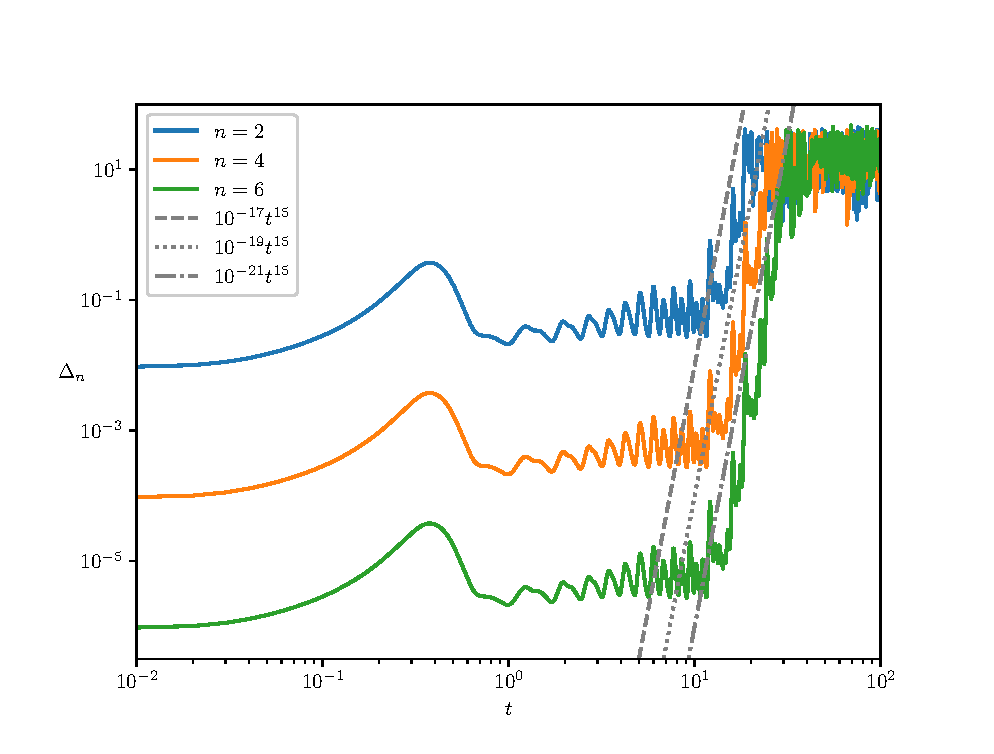
\includegraphics[width=1\hsize]{kadai7/2fulllog.eps}
                    \caption{
                        $\Delta_n(t)$の計算結果
                        (両対数グラフ)
                    }
                    \label{fig:7fulllog}
                \end{minipage}
            \end{figure}

        \subsubsection{考察}
            $\Delta_n(t)$の関数形を調べるために、
            冪関数と指数関数をそれぞれ図\ref{fig:7halflog}, \ref{fig:7fulllog}
            に重ねたグラフを図\ref{fig:7halflog_power}〜\ref{fig:7fulllog_exp}に示す。
            \begin{figure}[h]
                \begin{minipage}{0.49\hsize}
                    \centering
                    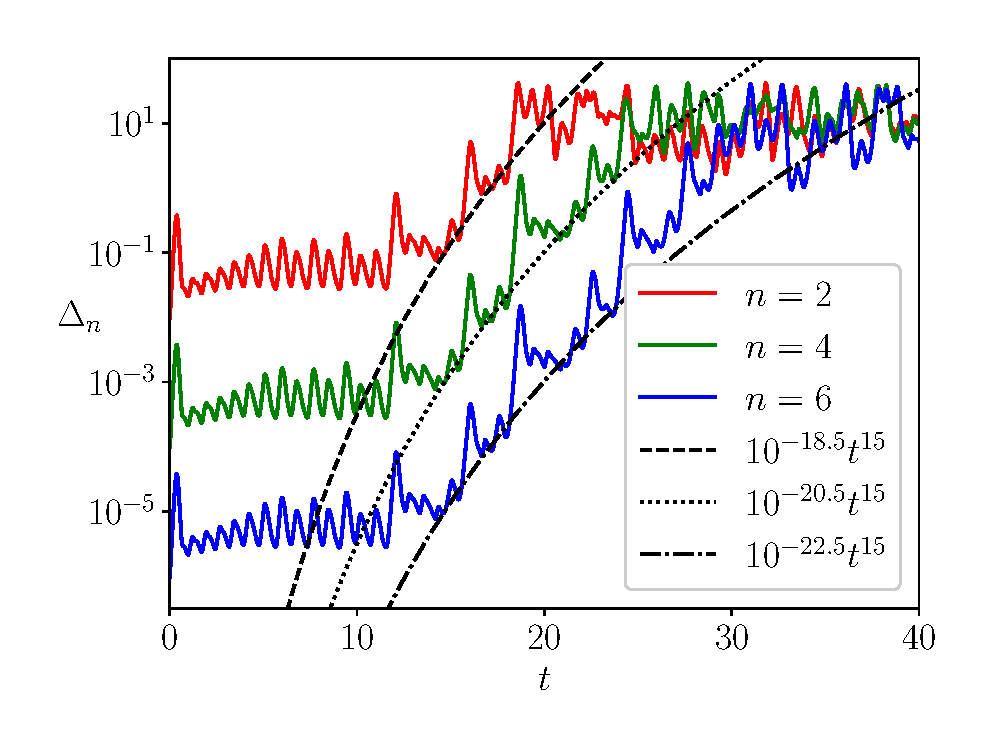
\includegraphics[width=1\hsize]{kadai7/2halflog_power.eps}
                    \caption{
                        $\Delta_n(t)$に冪関数を重ねた図(片対数グラフ)
                    }
                    \label{fig:7halflog_power}
                \end{minipage}
                \begin{minipage}{0.49\hsize}
                    \centering
                    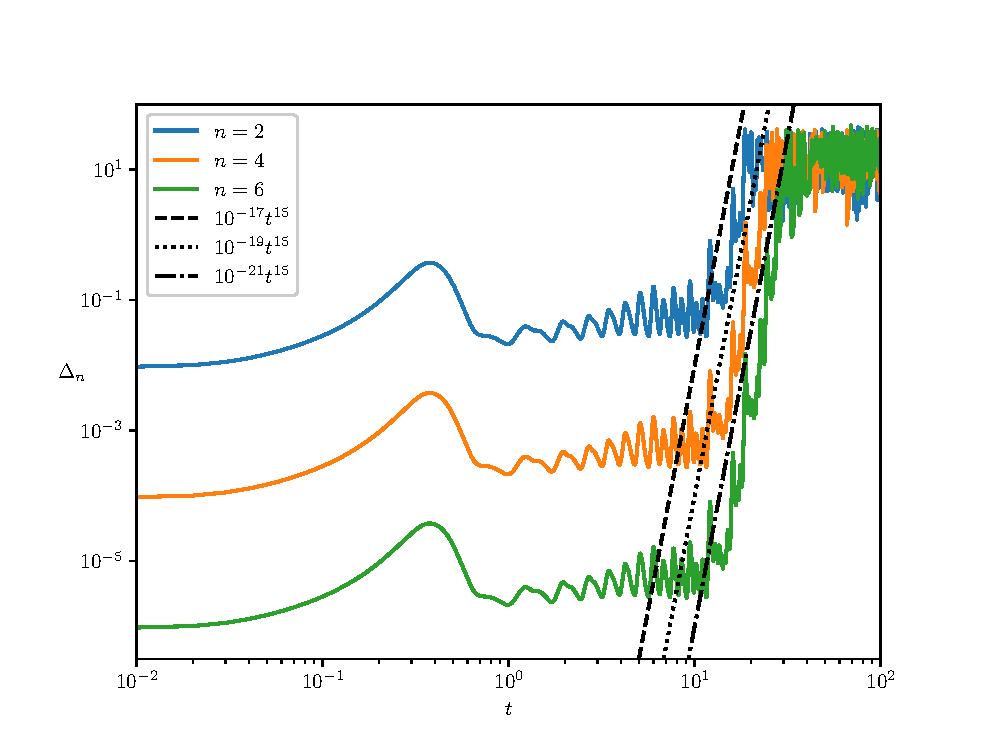
\includegraphics[width=1\hsize]{kadai7/2fulllog_power.eps}
                    \caption{
                        $\Delta_n(t)$に冪関数を重ねた図(両対数グラフ)
                    }
                    \label{fig:7fulllog_power}
                \end{minipage}
            \end{figure}
            \begin{figure}[h]
                \begin{minipage}{0.49\hsize}
                    \centering
                    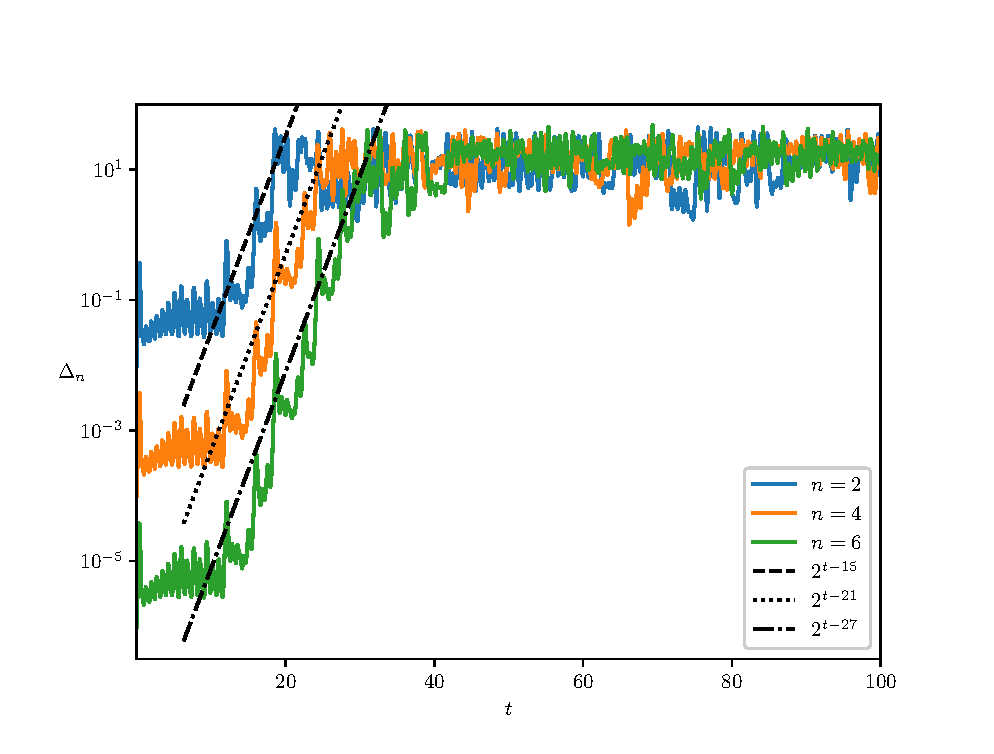
\includegraphics[width=1\hsize]{kadai7/2halflog_exp.eps}
                    \caption{
                        $\Delta_n(t)$に指数関数を重ねた図(片対数グラフ)
                    }
                    \label{fig:7halflog_exp}
                \end{minipage}
                \begin{minipage}{0.49\hsize}
                    \centering
                    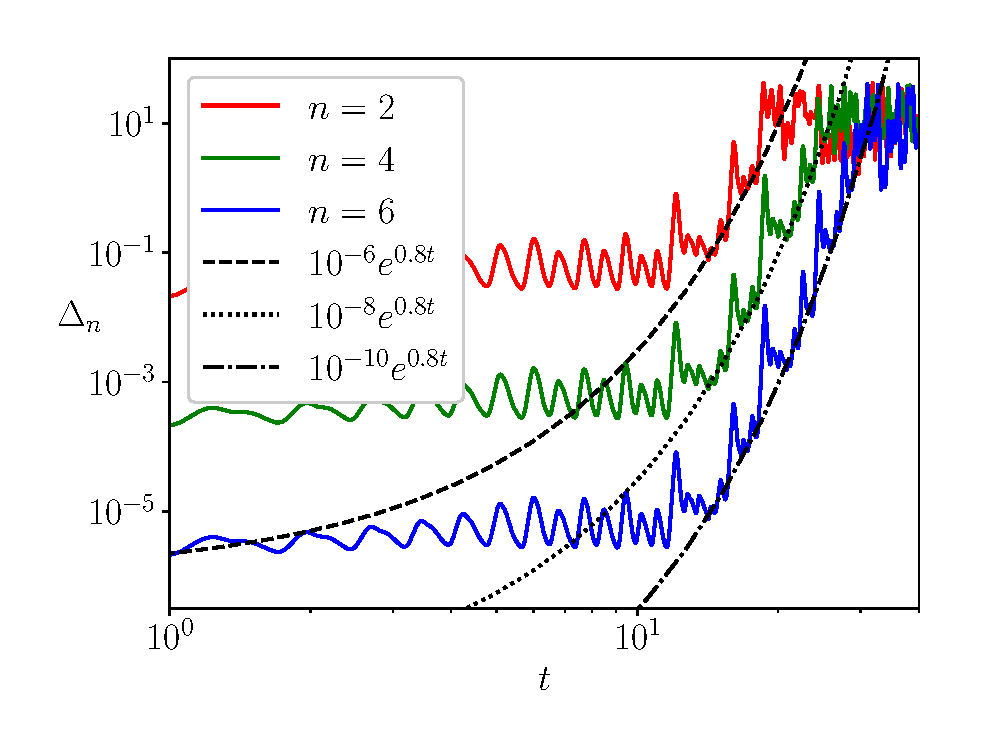
\includegraphics[width=1\hsize]{kadai7/2fulllog_exp.eps}
                    \caption{
                        $\Delta_n(t)$に指数関数を重ねた図(両対数グラフ)
                    }
                    \label{fig:7fulllog_exp}
                \end{minipage}
            \end{figure}
            図\ref{fig:7fulllog_power}, \ref{fig:7halflog_exp}を見ると、
            冪関数と指数関数のどちらも綺麗に重なっているように見える。
            しかし、図\ref{fig:7halflog_power}を見ると、
            $n$が増加するにつれ、漸近値付近で$\Delta_n(t)$と冪関数の差が開いていることがわかる。
            一方、図\ref{fig:7fulllog_exp}を見ると、
            指数関数は$n$が変化しても重なったままである。

            以上より、$\Delta_n(t)$の漸近値直前の関数形は指数関数であり、
            その指数は0.8であることがわかった。

        \subsubsection{結論}
            $\Delta_n(t)$の漸近値直前の関数形は$n$に依存せず、
            $e^{-0.8t}$である。

    \subsection{課題8 連立微分方程式}
        式(\ref{equ:sim})で表される連立微分方程式を考える。
        \begin{eqnarray}
            \frac{\mathrm{d}x_i}{\mathrm{d}t} &=& \omega_i - \frac{K}{N}\sum^N_{j=1}\sin(x_i-x_j) \label{equ:sim} \\
            \omega_i &\coloneqq& \tan\left\{\pi\left(\frac{i}{N + 1} - \frac{1}{2}\right)\right\} \ (i = 1, 2, \cdots, N) \nonumber
        \end{eqnarray}
        ここで、$K$は定数である。また、初期値は次式で与えられる。
        \begin{equation*}
            x_i(0) = y_i + 0.01\sin y_i, \ y_i \coloneqq \frac{i - 1}{N}2\pi \ (i = 1, 2, \cdots, N)
        \end{equation*}
        また、式(\ref{equ:order})で定義される値$R(t)$を考える。
        \begin{equation}
            R(t) = \sqrt{R_x^2 + R_y^2}, \ R_x \coloneqq \frac{1}{N}\sum^N_{j=1}\cos x_j, \ R_y \coloneqq \frac{1}{N}\sum^N_{j=1}\sin x_j \label{equ:order}
        \end{equation}

        ステップ幅$\Delta t = 0.01$の4次ルンゲ・クッタ法を用いて数値計算を行う。
        $N=10^2, 10^3$に対して、$t\in[50, 100]$の区間において$R(t)$の時間平均を以下で定義する。
        \begin{equation*}
            \bar{R} \coloneqq \frac{1}{50}\int^{100}_{50}R(t)dt
        \end{equation*}
        $K$を区間$[1, 3]$内で0.01刻みで動かし、
        $\bar{R}$を$K$の関数としてプロットする。

        \subsubsection{計算量の削減}
            式(\ref{equ:sim})をそのまま計算すると、
            $O(N^2)$の時間計算量を要するが、
            $O(N)$で計算する方法を述べる。

            右辺第2項の総和の中身に加法定理を適用すると、
            \begin{eqnarray*}
                \frac{K}{N}\sum^N_{j=1}\sin(x_i-x_j) &=& \frac{K}{N}\sum^N_{j=1}(\sin x_i\cos x_j - \cos x_i \sin x_j) \\
                &=& K\left(\sin x_i\frac{1}{N}\sum^N_{j=1}\cos x_j - \cos x_i\frac{1}{N}\sum^N_{j=1}\sin x_j\right) \\
                &=& K (R_x\sin x_i - R_y\cos x_i)
            \end{eqnarray*}
            となり、式(\ref{equ:sim})は
            \begin{equation*}
                \frac{\mathrm{d}x_i}{\mathrm{d}t} = \omega_i - K (R_x\sin x_i - R_y\cos x_i)
            \end{equation*}
            と書ける。これは$R_x, R_y$の前計算を行うことで$O(1)$で計算できるため、
            全体では$O(N)$の時間計算量となる。

        \subsubsection{結果}
            計算した$\bar{R}(K)$を図\ref{fig:8}に示す。
            \begin{figure}[h]
                \centering
                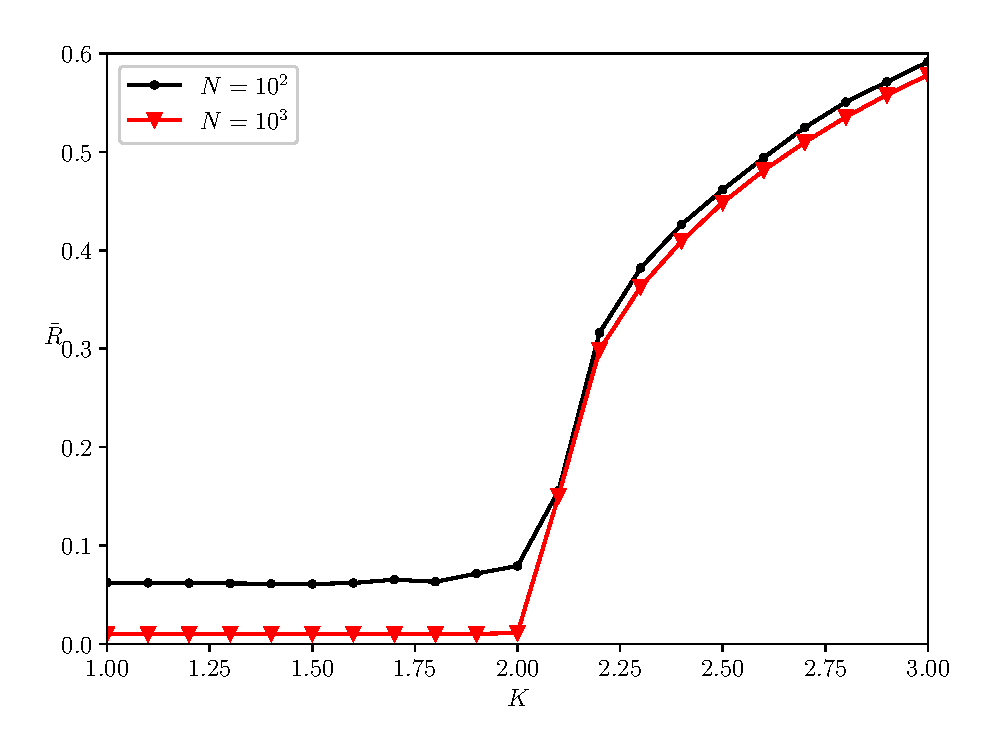
\includegraphics[width=0.8\hsize]{kadai8/8.eps}
                \caption{
                    計算した$\bar{R}(K)$。
                }
                \label{fig:8}
            \end{figure}

        \subsubsection{考察}
            $N\rightarrow\infty$とした際、$K=2$は臨界点と呼ばれている。
            その理由を以下に考察する。

            $x_i$を位相とすると、
            $xy$平面における単位円上のその位相を持つ点の座標は$(\cos x_i, \sin x_i)$と書ける。
            よって、式(\ref{equ:order})より、
            $R_x, R_y$はそれぞれ$N$点の$x, y$座標の平均であるといえ、
            $R$は平均座標のノルムである。

            以上を踏まえると、$x_i$の分散が大きいほど$R$は0に近づき、
            分散が小さいほど$R$は1に近づくことがわかる。
            図\ref{fig:k1}, \ref{fig:k3}に$N=10^2$について、
            $K=1, 3$のときの単位円上の$N$点$(\cos x_i(100), \sin x_i(100))$
            の分布を示す。
            \begin{figure}[h]
                \begin{minipage}{0.49\hsize}
                    \centering
                    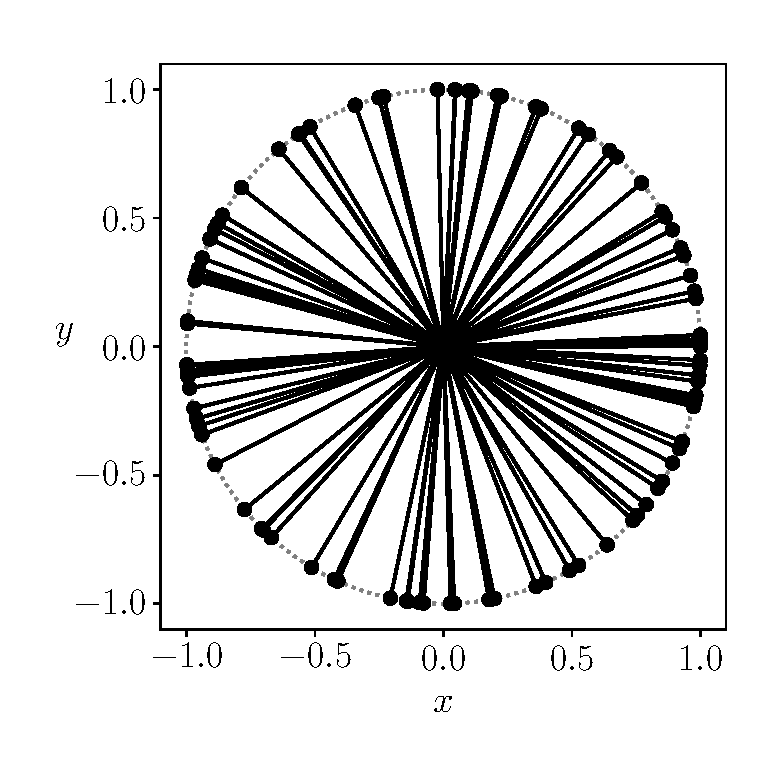
\includegraphics[width=1\hsize]{kadai8/K1.eps}
                    \caption{
                        $K=1$のときの$x_i \ (i\in 1, 2, \cdots,N)$の分布
                    }
                    \label{fig:k1}
                \end{minipage}
                \begin{minipage}{0.49\hsize}
                    \centering
                    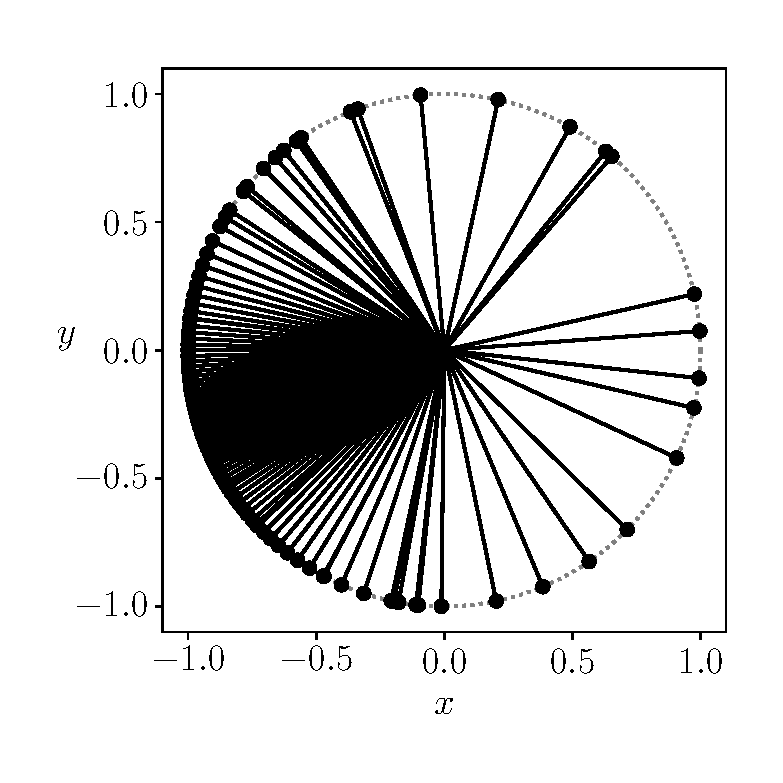
\includegraphics[width=1\hsize]{kadai8/K3.eps}
                    \caption{
                        $K=3$のときの$x_i \ (i\in 1, 2, \cdots,N)$の分布
                    }
                    \label{fig:k3}
                \end{minipage}
            \end{figure}
            図\ref{fig:8}と図\ref{fig:k1}, \ref{fig:k3}を見比べると、
            $\bar{R}\approx 0$である$K=1$のときは実際に$x_i$の分散が大きく、
            逆に$\bar{R}$が増加している$K=3$のときは$x_i$の分散が小さいことがわかる。

            また、図\ref{fig:8}より、$N = 10^2, 10^3$のどちらについても、
            $K \leq 2$のときは$R\approx 0$で、
            $K > 2$のときに$R$が増加していることわかり、
            これが$K = 2$が臨界点と呼ばれる要因であると考えられる。

\section{付録}
    本節には\ref{sec:ex}節で作成したc++コードを一部抜粋して記述する。

    \subsection{課題3}
        \begin{lstlisting}[caption=前進オイラー法]
const double euler(
    const double (*f)(double , double), // 被積分関数
    double u, // 初期値
    const double dt, // ステップ幅
    const double start, const double end // 積分範囲
) {
    for (double t = start; t < end; t += dt)
        u += f(t, u) * dt;

    return u;
}
        \end{lstlisting}
        \begin{lstlisting}[caption=2次アダムス・バッシュフォース法]
const double adams_second(
    const double (*f)(double , double), // 被積分関数
    const double (*uexact)(double), // 厳密解
    double u, // 初期値
    const double dt, // ステップ幅
    const double start, const double end // 積分範囲
) {
    double lastf = uexact(start - dt);
    for (double t = start; t < end; t += dt) {
        const double nowf = f(t, u);
        u += (3.0 * nowf - lastf) * dt / 2.0;

        lastf = nowf;
    }

    return u;
}
        \end{lstlisting}
        \begin{lstlisting}[caption=3次アダムス・バッシュフォース法]
const double adams_third(
    const double (*f)(double , double), // 被積分関数
    const double (*uexact)(double), // 厳密解
    double u, // 初期値
    const double dt, // ステップ幅
    const double start, const double end // 積分範囲
) {
    double lastf = uexact(start - dt), lastlastf = uexact(start - dt - dt);
    for (double t = start; t < end; t += dt) {
        const double nowf = f(t, u);
        u += (23.0 * nowf - 16.0 * lastf + 5.0 * lastlastf) * dt / 12.0;

        lastlastf = lastf; lastf = nowf;
    }

    return u;
}
        \end{lstlisting}
        \begin{lstlisting}[caption=ホイン法, label=src:heun]
const double heun(
    const double (*f)(double , double), // 被積分関数
    double u, // 初期値
    const double dt, // ステップ幅
    const double start, const double end // 積分範囲
) {
    for (double t = start; t < end; t += dt)
        u += (f(t, u) + f(t + dt, u + f(t, u) * dt)) * dt / 2.0;

    return u;
}
        \end{lstlisting}
        \begin{lstlisting}[caption=4次ルンゲ・クッタ法]
const double runge_kutta(
    const double (*f)(double , double), // 被積分関数
    double u, // 初期値
    const double dt, // ステップ幅
    const double start, const double end // 積分範囲
) {
    for (double t = start; t < end; t += dt) {
        const double f1 = f(t, u);
        const double f2 = f(t + dt / 2.0, u + f1 * dt / 2.0);
        const double f3 = f(t + dt / 2.0, u + f2 * dt / 2.0);
        const double f4 = f(t + dt, u + f3 * dt);

        u += (f1 + 2 * f2 + 2 * f3 + f4) * dt / 6.0;
    }

    return u;
}
        \end{lstlisting}

    \subsection{課題4}
        \begin{lstlisting}[caption=クランク・ニコルソン法]
constexpr double ALPHA = 10;
constexpr double BETA = 1;

void crank(
    const double (*f)(double , double), // 被積分関数
    double u, // 初期値
    const double dt, // ステップ幅
    const double start, const double end // 積分範囲
) {
    double t;
    for (t = start; t < end; t += dt) {
        u = ((2.0 - ALPHA * dt) * u + 2.0 * BETA * dt) / (2.0 + ALPHA * dt);
    }
}
        \end{lstlisting}
        ホイン法はコード\ref{src:heun}と同じため、略。

    \subsection{課題5}
        \begin{lstlisting}[caption=式(\ref{equ:5alg})による数値計算]
void simulate(
    const double (*f)(double , double), // 被積分関数
    const double (*uexact)(double), // 厳密解
    double u, // 初期値
    const double dt, // ステップ幅
    const double start, const double end // 積分範囲
) {
    double lastu = uexact(start - dt);
    for (double t = start; t < end; t += dt) {
        const double utemp = u;
        u = lastu + 2 * dt * f(t, u);

        lastu = utemp;
    }
}
        \end{lstlisting}

    \subsection{課題7}
        \begin{lstlisting}[caption=4次ルンゲ・クッタ法によるローレンツ方程式の数値計算]
void runge_kutta(
    const double (*fx)(double , double, double),
    const double (*fy)(double , double, double),
    const double (*fz)(double , double, double), // 被積分関数
    double x, double y, double z, // 初期値
    const double dt, // ステップ幅
    const double start, const double end // 積分範囲
) {
    for (double t = start; t < end; t += dt) {
        const double fx1 = fx(x, y, z);
        const double fy1 = fy(x, y, z);
        const double fz1 = fz(x, y, z);

        const double fx2 = fx(x + fx1 * dt / 2.0, y + fy1 * dt / 2.0, z + fz1 * dt / 2.0);
        const double fy2 = fy(x + fx1 * dt / 2.0, y + fy1 * dt / 2.0, z + fz1 * dt / 2.0);
        const double fz2 = fz(x + fx1 * dt / 2.0, y + fy1 * dt / 2.0, z + fz1 * dt / 2.0);

        const double fx3 = fx(x + fx2 * dt / 2.0, y + fy2 * dt / 2.0, z + fz2 * dt / 2.0);
        const double fy3 = fy(x + fx2 * dt / 2.0, y + fy2 * dt / 2.0, z + fz2 * dt / 2.0);
        const double fz3 = fz(x + fx2 * dt / 2.0, y + fy2 * dt / 2.0, z + fz2 * dt / 2.0);

        const double fx4 = fx(x + fx3 * dt, y + fy3 * dt, z + fz3 * dt);
        const double fy4 = fy(x + fx3 * dt, y + fy3 * dt, z + fz3 * dt);
        const double fz4 = fz(x + fx3 * dt, y + fy3 * dt, z + fz3 * dt);

        x += (fx1 + 2 * fx2 + 2 * fx3 + fx4) * dt / 6.0;
        y += (fy1 + 2 * fy2 + 2 * fy3 + fy4) * dt / 6.0;
        z += (fz1 + 2 * fz2 + 2 * fz3 + fz4) * dt / 6.0;   
    }
}
        \end{lstlisting}

    \subsection{課題8}
        \begin{lstlisting}[caption=4次ルンゲ・クッタ法による$\bar{R}(K)$の計算]
#include <cmath>
#include <vector>

double runge_kutta(
    const double (*f)(double, int, double, int, double, double), // 被積分関数
    std::vector<double> x, // 初期値
    const double K, // 定数
    const int N, // 元数
    const double dt, // ステップ幅
    const double start, const double end, // 積分範囲
    double calc_t // 平均の計算開始時刻
) {
    double Rx, Ry;
    double Rsum = 0;
    for (double t = start; t < end; t += dt) {
        Rx = Ry = 0;
        for (int i = 0; i < N; i++) {
            Rx += cos(x[i]) / N;
            Ry += sin(x[i]) / N;
        }

        for (int i = 0; i < N; i++) {
            const double f1 = f(x[i], i, K, N, Rx, Ry);
            const double f2 = f(x[i] + f1 * dt / 2.0, i, K, N, Rx, Ry);
            const double f3 = f(x[i] + f2 * dt / 2.0, i, K, N, Rx, Ry);
            const double f4 = f(x[i] + f3 * dt, i, K, N, Rx, Ry);

            x[i] += (f1 + 2 * f2 + 2 * f3 + f4) * dt / 6.0;
        }

        if (t >= calc_t) {
            Rsum += sqrt(Rx * Rx + Ry * Ry) * dt;
        }
    }

    return Rsum / (end - calc_t);
}

void calculate_Rbar(
    int N // 元数
) {
    const double start = 0, end = 100, calc_t = 50, dt = 0.01;
    std::vector<double> x(N);
    for (int i = 0; i < N; i++) {
        const double y = 2 * M_PI / N * (i - 1);
        x[i] = y + 0.01 * sin(y);
    }

    for (double K = 1; K <= 5 + 1e-7; K += 0.1)
        const double R = runge_kutta(f, x, K, N, dt, start, end, calc_t);
}
        \end{lstlisting}

\newpage
\addcontentsline{toc}{section}{参考文献}
\begin{thebibliography}{99}
    \bibitem{text}{
        実験演習ワーキンググループ、``数理工学実験 2022年度版''、京都大学工学部情報学科数理工学コース (2022)
    }
    \bibitem{runge}{
        斉藤宣一、``数値解析入門''、東京大学出版 (2012)
    }
    \bibitem{2rec}{
        高校数学の美しい物語、``$f(n)$を含む二項間漸化式の2通りの解法''、\\
        ``https://manabitimes.jp/math/687'', (最終更新: 2021/3/7)
    }
    \bibitem{3rec}{
        高校数学の美しい物語、``三項間漸化式の3通りの解き方''、\\
        ``https://manabitimes.jp/math/697'', (最終更新: 2021/3/7)
    }
\end{thebibliography}
\end{document}